В том случае если рентгеновское излучение отражается от атомных плоскостей не
 параллельных поверхности, в таком случае говорят об асимметрии отражения (рисунок ~\ref{ris:assymetric_brag}).

\begin{figure}[h]
  \centering
  \subfloat[$b >> 1$, $\varphi$ > 0]{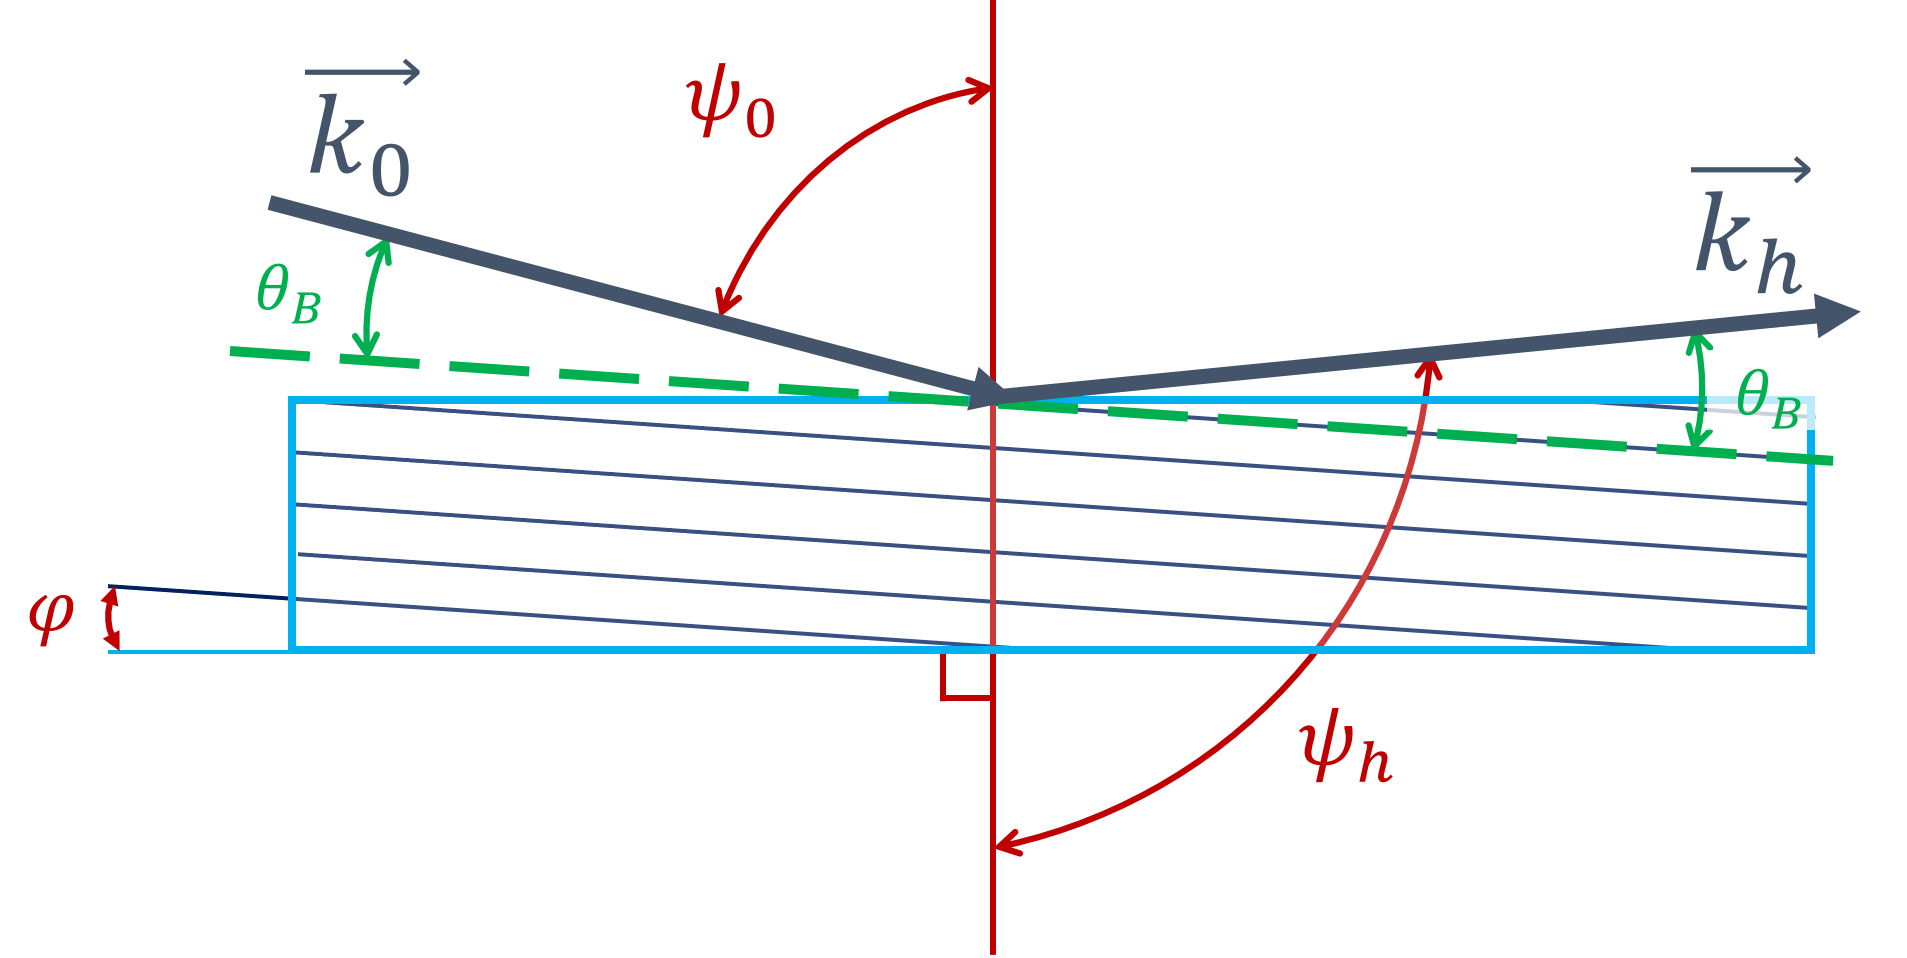
\includegraphics[width=0.45\textwidth]{images/assym2.png}\label{fig:f1}}
  \hfill
  \subfloat[$b << 1$, $\varphi$ < 0]{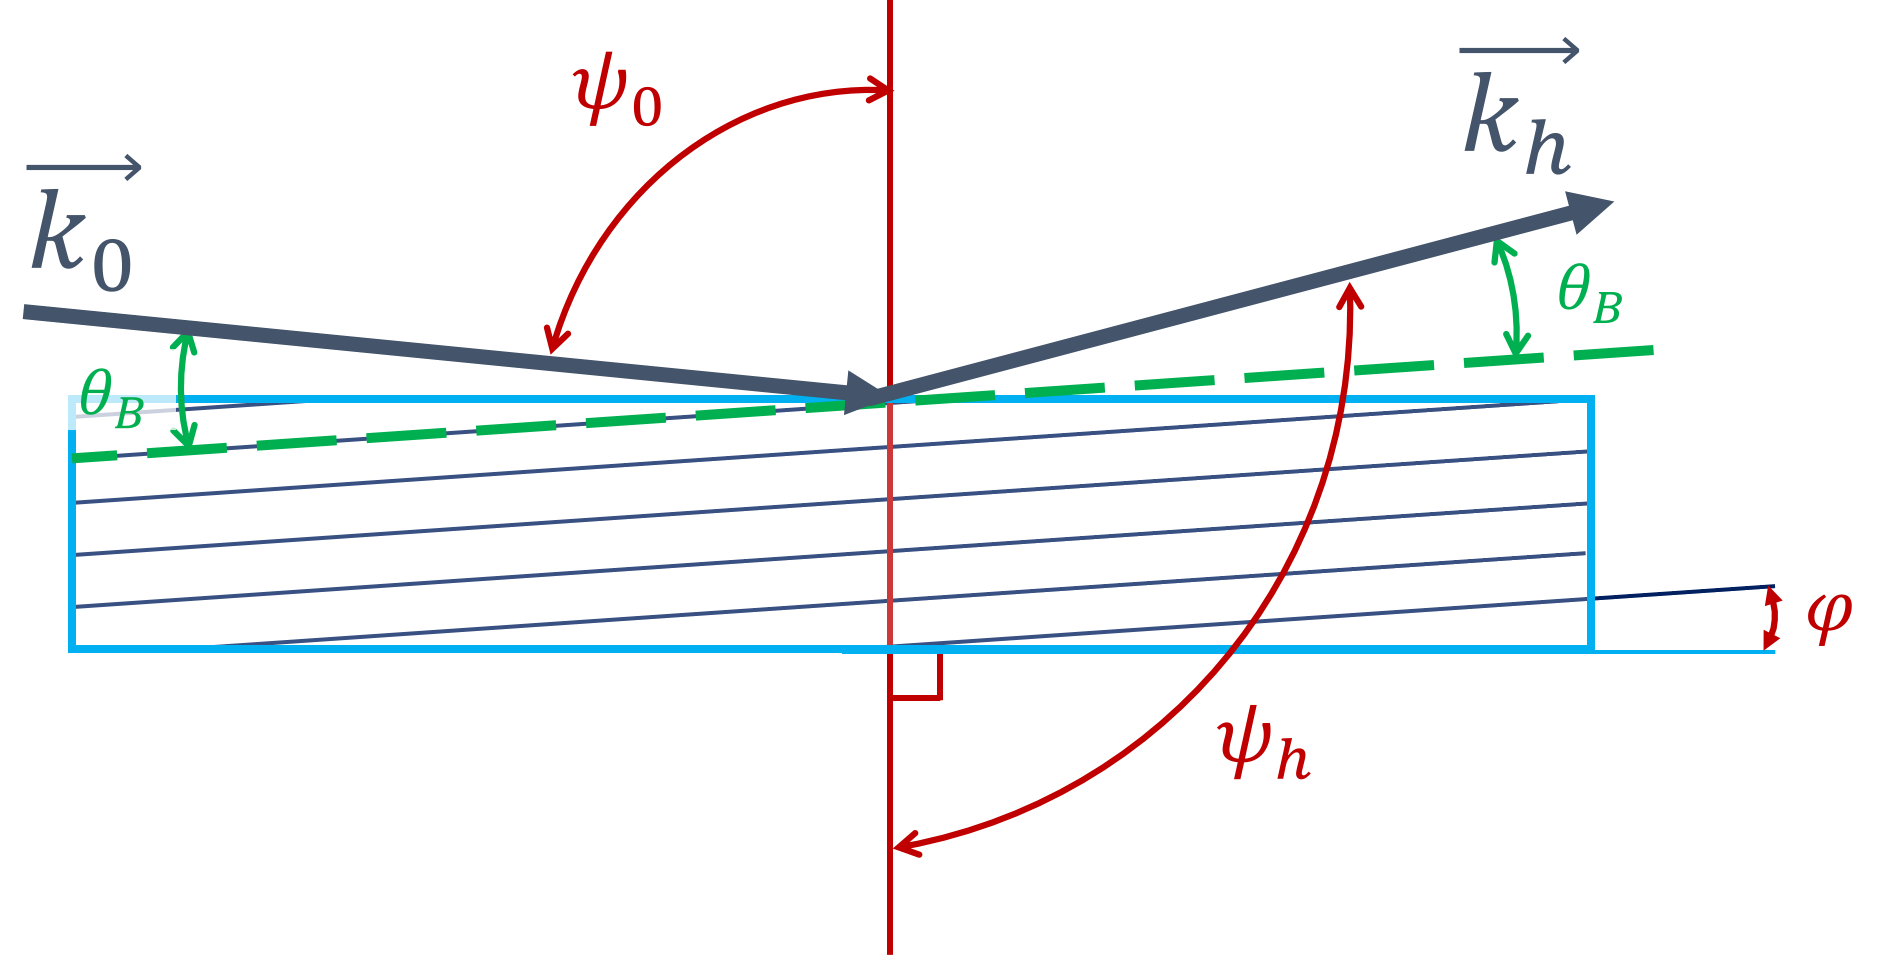
\includegraphics[width=0.45\textwidth]{images/assym1.png}\label{fig:f2}}
  \caption{Схема Брегговской дифракции для асимметричного отражения}
  \label{ris:assymetric_brag}
\end{figure}

Для того чтобы охарактеризовать степень асимметрии, введем коэффициент $b$:

\begin{equation}
  b = \frac {\gamma_0}{|\gamma_h|}
  \label{eq:koef_b}
 \end{equation}
где, $\gamma_0 = cos \psi_0 = sin ( \varphi + \theta_B)$, $\gamma_h = cos \psi_h = sin ( \varphi - \theta_B)$,
$\varphi$ - угол между плоскостью отражения и поверхностью образца.
